

Per confrontare i dati sperimentali con la (5), sono state effettuate misure della temperatura ambiente, indicata con $T_2$, e della temperatura intermedia, indicata con $T(t)$, ad istanti di tempo distinti e riportati in tabella:

\begin{table}[H]
	\centering
	\begin{tabular}{|c|}
		\hline
		\textbf{t $[s]$} \\
		\hline
		$5\pm 0.05$ \\
		$8\pm 0.05$ \\
		$11\pm 0.05$ \\
		$14\pm 0.05$ \\
		$17\pm 0.05$ \\
            $20\pm 0.05$ \\
            $23\pm 0.05$ \\
            $26\pm 0.05$ \\
		\hline
	\end{tabular}
	\caption{Istanti di tempo utilizzati per misurare il valore della           temperatura intermedia $T(t)$.}
	\label{tab:}
\end{table}
La procedura è stata ripetuta 4 volte.
\begin{table}[H]
\centering
\begin{tabular}{|c|c|c|c|c|c|c|c|c|}
\hline
\textbf{s} & \textbf{$T_1$} & \textbf{$T_2$} & \textbf{$T_1$} & \textbf{$T_2$} & \textbf{$T_1$} & \textbf{$T_2$} & \textbf{$T_1$} & \textbf{$T_2$} \\
\hline
5.00 & 22.7 & 55 & 23.8 & 56 & 24.4 & 57 & 24.8 & 60 \\
8.00 & 22.3 & 46 & 24.1 & 44 & 24.6 & 48 & 24.9 & 49 \\
11.00 & 23.1 & 38 & 24.3 & 40 & 24.7 & 41 & 25.2 & 40 \\
14.00 & 22.9 & 34 & 24.1 & 35 & 24.7 & 35 & 25.2 & 35 \\
17.00 & 22.5 & 31 & 24.3 & 33 & 24.7 & 33 & 25.1 & 34 \\
20.00 & 22.9 & 29 & 24.3 & 30 & 24.8 & 31 & 25.1 & 32 \\
23.00 & 22.8 & 28 & 24.3 & 29 & 24.8 & 29.5 & 25.2 & 30 \\
26.00 & 23.1 & 27 & 24.4 & 28 & 24.8 & 29 & 25.2 & 29.5 \\
\hline
\end{tabular}
\caption{Tabella aggregata di tutte le misure dirette. L'errore assoluto sui secondi è di $\pm 0.01s$, mentre sui tempi $T_1$ e $T_2$ è di $\pm 0.1\,^\circ\mathrm{C}$.}
\label{tab:esempio}
\end{table}
Per ciascuna prova i dati sperimentali sono stati riportati, previa linearizzazione della (3), su un grafico che contiene anche una retta dei minimi quadrati:
\begin{figure}[H]
	\centering
	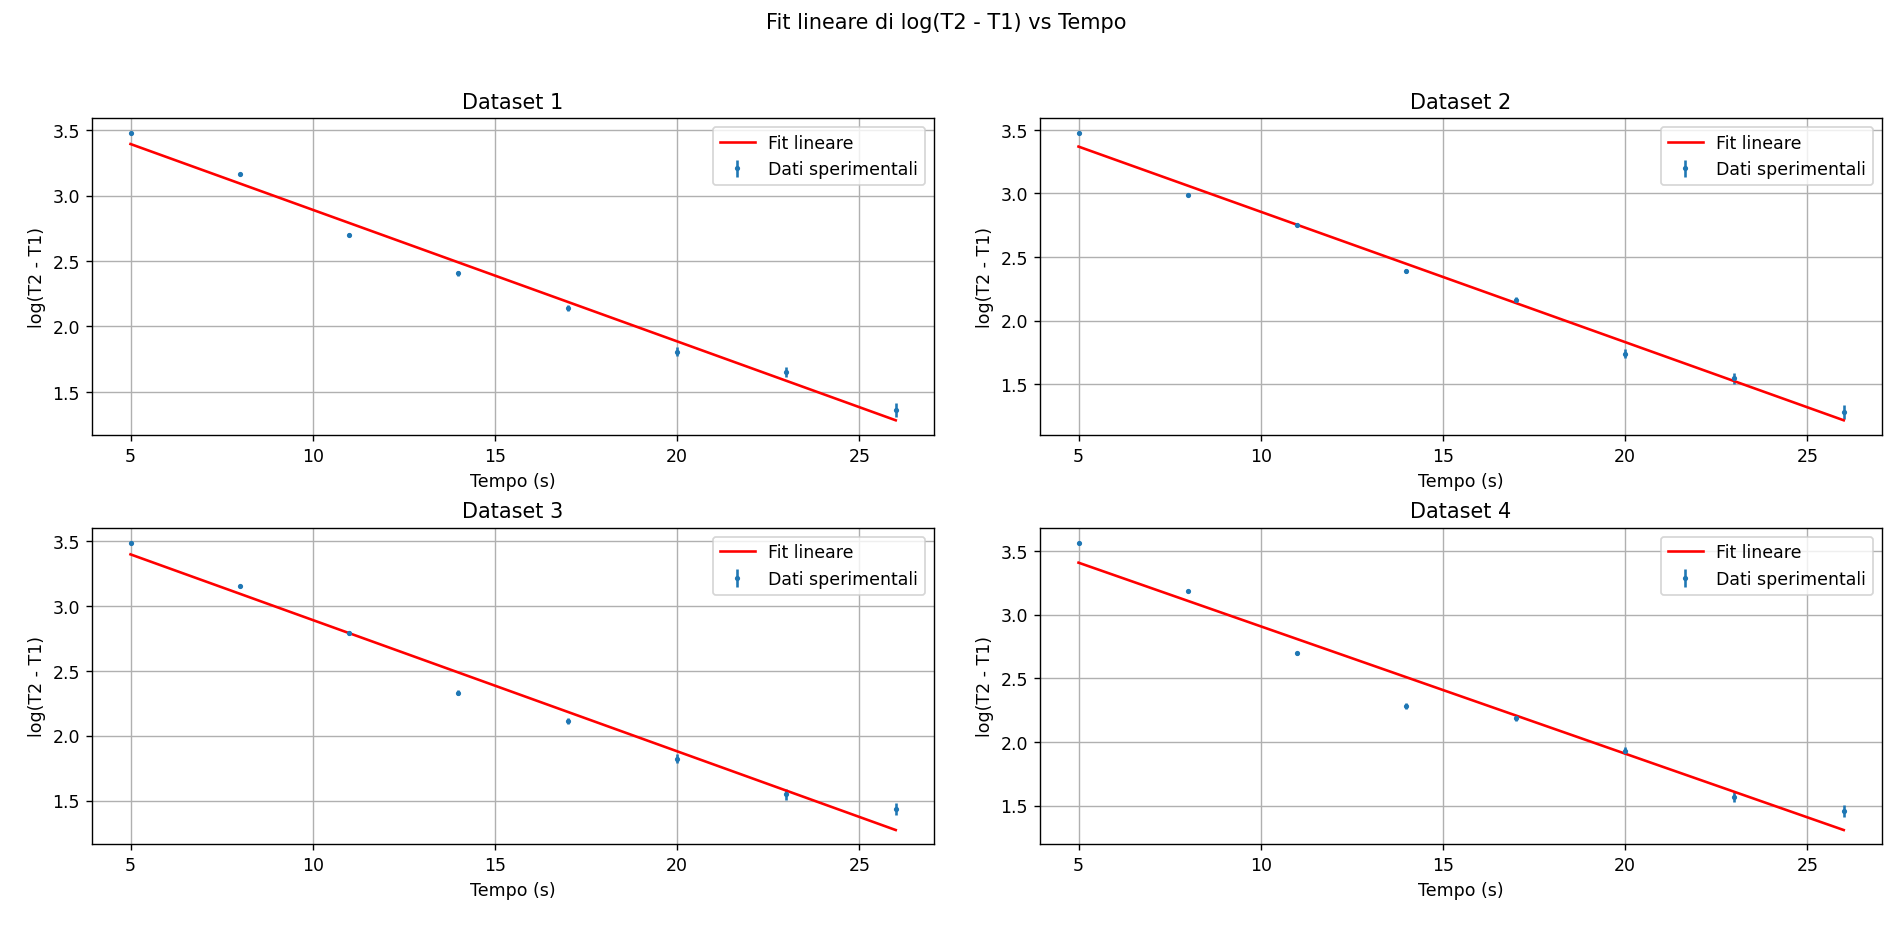
\includegraphics[width=1\textwidth]{./graph.png}
	\caption{}
\end{figure} 
Tra i vari fit, il migliore appare essere quello relativo al Dataset 2, da cui ricaviamo un coefficiente angolare pari a:
\begin{equation}
    b = -0.10 \pm 0.01 s
\end{equation}
Ricordando che la costante di tempo $\tau$ e il coefficiente angolare $b$ sono legati dalla seguente relazione:
\begin{equation}
    b = -\frac{1}{\tau}
\end{equation}
si ottiene il seguente valore per $\tau = 10.00s$. L'incertezza su $\tau$ è fornita dalla legge:
\begin{align}
    \delta \tau &= \left| \frac{d}{b}(-\frac{1}{b}) \right| \ \delta b  \\
    &= \left| \frac{1}{b^2} \right| \ \delta b = \\
    &= 1.00s
\end{align}